\section*{Đề thi thử liên trường THPT Nghệ 25-26 - lần 2}

\caulc
\Opensolutionfile{ans}[ans/ans-26-20-lientruongNgheAn-L2-LC]
\begin{ex}%[0H9N4-1]
	Trong mặt phẳng $Oxy$, cho đường tròn $(C)$ có phương trình $(x+2)^2+(y-3)^2=5$. Tọa độ tâm và bán kính của đường tròn $(C)$ là
	\choice
	{\True $I(-2;3)$, $R=\sqrt{5}$}
	{$I(2;-3)$, $R=5$}
	{$I(2;-3)$, $R=\sqrt{5}$}
	{$I(-2;3)$, $R=5$}
	\loigiai{
		Đường tròn $(C)$ có tâm $I(-2;3)$ và bán kính $R=\sqrt{5}$.
	}
\end{ex}
\begin{ex}%[2D1H5-1]
	Cho hàm số $y=\dfrac{ax+2}{x+c}$ có đồ thị như hình sau đây.
	\begin{center}
		\begin{tikzpicture}[line join=round, line cap=round,>=stealth,scale=.7]
			\tikzset{every node/.style={scale=0.8}}
			\draw[->] (-5,0)--(7,0) node[below left] {$x$};
			\draw[->] (0,-5)--(0,6) node[below left] {$y$};
			\draw (0,0) node [below left] {\footnotesize $O$};
			\draw[fill=black] (2,0) circle (1.2pt) node [below right] {\footnotesize $2$};
			\draw[fill=black] (-2,0) circle (1.2pt) node [below] {\footnotesize $-2$};
			\draw [fill=black] (0,1) circle (1.2pt) node [above right] {\footnotesize $1$};
			\draw [fill=black] (0,-1) circle (1.2pt) node [above right] {\footnotesize $-1$};
			\begin{scope}
				\clip (-5,-5) rectangle (7,6);
				\draw[samples=200,domain=-5:1.9,smooth,variable=\x]
				plot (\x,{(1*(\x)+2)/(1*(\x)-2)});
				\draw[samples=200,domain=2.1:7,smooth,variable=\x]
				plot (\x,{(1*(\x)+2)/(1*(\x)-2)});
				\draw[dashed,samples=200,domain=-5:9,smooth,variable=\x]
				plot (\x,{(1.0});
				\draw[dashed] (2.0,-5)--(2.0,6);
			\end{scope}
		\end{tikzpicture}
	\end{center}
	Tính giá trị của biểu thức $P=2a-c$.
	\choice
	{\True $4$}
	{$-4$}
	{$-5$}
	{$5$}
	\loigiai{
		Điều kiện $x \neq -c$ \\
		Theo giả thiết bài toán, ta có \\
		Đường tiệm cận đứng $x=-c$. \\
		Đường tiệm cận ngang $y=a$. \\
		Theo đồ thị, ta có $\heva{&-c=2\\ &a=1} \Rightarrow \heva{&c=-2\\ &a=1.}$\\
		Vậy $2a-c=2\cdot1-(-2)=4$.
	}
\end{ex}
\begin{ex}%[1H4N5-3]
	Cho hình hộp $ABCD.A'B'C'D'$.
	\begin{center}
		\begin{tikzpicture}[declare function={goc=220; gocx=80; a=3; b=5; h=4;},scale=.7,font=\footnotesize,line join=round
			,line cap=round,>=stealth]
			\path
			(0,0) coordinate (A)
			(b,0) coordinate (B)
			(goc:a) coordinate (D)
			($(D)+(B)-(A)$) coordinate (C)
			(gocx:h) coordinate (A')
			($(gocx:h)+(B)$) coordinate (B')
			($(gocx:h)+(D)$) coordinate (D')
			($(gocx:h)+(C)$) coordinate (C');
			\draw[dashed] (D)--(A)--(B) (A)--(A');
			\draw (D)--(C)--(B)--(B')--(A')--(D')--(C')--(C) (D)--(D') (B')--(C');
			\foreach \x/\g in {A/135, B/0, C/0, D/180, A'/135, B'/30, C'/-15, D'/180 }{\draw[fill=black] (\x) circle (1pt) node[shift={(\g:7pt)},font=\footnotesize]{$\x$};}
		\end{tikzpicture}
	\end{center}
	Chọn đẳng thức đúng
	\choice
	{$\overrightarrow{AC'} = \overrightarrow{AB} + \overrightarrow{AB'} + \overrightarrow{AD}$}
	{$\overrightarrow{DB'} = \overrightarrow{DA} + \overrightarrow{DD'} + \overrightarrow{DB}$}
	{\True $\overrightarrow{DB'} = \overrightarrow{DA} + \overrightarrow{DD'} + \overrightarrow{DC}$}
	{$\overrightarrow{AC'} = \overrightarrow{AC} + \overrightarrow{AB} + \overrightarrow{AD}$}
	\loigiai{
		Theo quy tắc hình hộp ta có $\overrightarrow{DB'} = \overrightarrow{DA} + \overrightarrow{DD'} + \overrightarrow{DC}$.
	}
\end{ex}
\begin{ex}%[2H2H1-1]
	Trong không gian với hệ tọa độ $Oxyz$, cho điểm $M$ có hình chiếu vuông góc lên mặt phẳng $(Oxy)$ và $(Oxz)$ lần lượt là $M_1(-2;3;0)$ và $M_2(-2;0;5)$. Tọa độ điểm $M$ là
	\choice
	{$M(-2;-3;5)$}
	{$M(2;-3;5)$}
	{$M(2;-5;3)$}
	{\True $M(-2;3;5)$}
	\loigiai{
		Do hình chiếu vuông góc của $M$ lên $(Oxy)$ là $M_1(-2;3;0)$ nên $x_M=-2$ và $y_M=3$.\\
		Do hình chiếu vuông góc của $M$ lên mặt phẳng $(Oxz)$ là $M_2(-2;0;5)$ nên $z_M=5$.\\
		Vậy điểm $M(-2;3;5)$.
	}
\end{ex}
\begin{ex}%[2H2H1-2]
	Trong không gian với hệ trục tọa độ $Oxyz$, cho hai vectơ $\vec{a}=(1;-2;1)$,
	$\vec{b}=(-2;1;1)$. Góc giữa hai vectơ $\overrightarrow{a}$ và $\vec{b}$ là
	\choice
	{$30^\circ$}
	{\True $120^\circ$}
	{$60^\circ$}
	{$150^\circ$}
	\loigiai{
		Ta có $\cos(\vec{a},\vec{b}) = \dfrac{\vec{a}\cdot\vec{b}}{|\vec{a}|\cdot|\vec{b}|} = \dfrac{1\cdot(-2)+(-2)\cdot1+1\cdot 1}{\sqrt{1^2+(-2)^2+1^2}\cdot\sqrt{(-2)^2+1^2+1^2}} = -\dfrac{1}{2}$.\\
		Vậy $(\overrightarrow{a},\overrightarrow{b}) = 120^\circ$.
	}
\end{ex}
\begin{ex}%[2D1V3-6]
	Bạn Hải có một tấm bìa hình vuông cạnh $40$ (cm). Bạn muốn cắt bỏ ở bốn góc bốn hình vuông nhỏ bằng nhau để gấp và dán lại thành một hình hộp chữ nhật không có nắp (tham khảo hình vẽ).
	\begin{center}
		\begin{tikzpicture}[scale=.7, line join = round, line cap = round]
			\tikzset{label style/.style={font=\footnotesize}}
			\def\a{5.5}
			\path 	(0:0) coordinate (A)
			++(0:\a) coordinate (B)
			++(90:\a) coordinate (C)
			($(A)-(B)+(C)$) coordinate (D)
			($(A)+(45:.35*\a)$) coordinate (A')
			($(B)+(135:.35*\a)$) coordinate (B')
			($(C)+(-135:.35*\a)$) coordinate (C')
			($(D)+(-45:.35*\a)$) coordinate (D')
			($(A)+(0:.35*\a)$) coordinate (E);
			\draw[dashed] 	(A')--(B')--(C')--(D')--cycle;
			\draw	(A)--(B)--(C)--(D)--cycle;
			\draw[pattern=north west lines] (A) rectangle (A')	(B) rectangle (B')	(C) rectangle (C')	(D) rectangle (D');
		\end{tikzpicture}\hspace{2cm}
		\begin{tikzpicture}[scale=1, line join = round, line cap = round]
			\def\a{3}
			\def\b{1.5}
			\def\h{1.3}
			\path 	(0:0) coordinate (A)
			++(0:\a) coordinate (D)
			++(-150:\b) coordinate (C)
			($(A)+(C)-(D)$) coordinate (B)
			($(A)+(90:\h)$) coordinate (A')
			($(B)+(90:\h)$) coordinate (B')
			($(C)+(90:\h)$) coordinate (C')
			($(D)+(90:\h)$) coordinate (D');
			\draw[dashed] 	(B)--(A)--(D)	(A)--(A');
			\draw 	(C)--(C') 	(D)--(D') 	(B)--(B')	(C)--(C')
			(B)--(C)--(D)
			(A')--(B')--(C')--(D')--cycle;
		\end{tikzpicture}
	\end{center}
	Để hộp có thể tích lớn nhất thì độ dài cạnh của hình vuông nhỏ bị cắt là
	\choice
	{$6$ (cm)}
	{$5$ (cm)}
	{\True $\dfrac{20}
		{3}$ (cm)}
	{$\dfrac{10}{3}$ (cm)}
	\loigiai{
		Cạnh hình vuông nhỏ có độ dài là $x$ (cm), với $0 < x < 20$.\\
		Hình hộp chữ nhật có cạnh đáy là $(40-2x)$ $(cm)$ và chiều cao là $x$ (cm).\\
		Thể tích của khối hộp là $V(x) = x(40-2x)^2 = 4x^3 - 160x^2 + 1600x$.\\
		Ta có $V'(x) = 12x^2 - 320x + 1600$.\\
		$V'(x) = 0 \Leftrightarrow \hoac{&x_1 = 20 \\&x_2 = \dfrac{20}{3}.}$ \\
		Ta có bảng biến thiên sau đây
		\begin{center}
			
\begin{tikzpicture} [scale=.7,font=\footnotesize,line join=round
				,line cap=round,>=stealth]
				\tkzTabInit[nocadre=false,deltacl=0.8, lgt=1.4, espcl=3.3]
				{$x$ /1.3,$V'(x)$/1,$V(x)$ /2.5}
				{$0$, $\dfrac{20}{3}$, $20$}
				\tkzTabLine{,+,0,-}
				\tkzTabVar{-/$V(0)$ , +/ $V\left(\dfrac{20}{3}\right)$ /, -/$V(20)$ /}
			\end{tikzpicture}
		\end{center}
		Do đó $\displaystyle\max\limits_{(0;20)} V(x) = V\left(\dfrac{20}{3}\right) = \dfrac{128\,000}{27}$.\\
		Vậy để hộp có thể tích lớn nhất thì độ dài cạnh của hình vuông nhỏ bị cắt là $\dfrac{20}{3}$ (cm).
	}
\end{ex}
\begin{ex}%[2D1N1-1]
	Hàm số nào sau đây nghịch biến trên $\mathbb{R}$?
	\choice
	{$y = \left(\dfrac{2026}
		{2025}\right)^x$}
	{$y = \log_{\dfrac{1}
			{2}} x$}
	{$y = \dfrac{2x-1}{x-1}$}
	{\True $y = e^{-x}$}
	\loigiai{
		\begin{itemize}
			\item Hàm số mũ $y = \left(\dfrac{2026}{2025}\right)^x$ có cơ số $\dfrac{2026}{2025} > 1$ nên hàm số đồng biến trên $\mathbb{R}$.
			\item Hàm số $y = \log_{\frac{1}{2}} x$ chỉ xác định khi $x > 0$ nên không thể nghịch biến trên $\mathbb{R}$.
			\item Hàm số $y = \dfrac{2x-1}{x-1}$ xác định khi $x \neq 1$ nên không thỏa mãn đầu bài.
			\item Hàm số $y = e^{-x} = \left(\dfrac{1}{e}\right)^x$ có cơ số $\dfrac{1}{e} < 1$ nên nghịch biến trên $\mathbb{R}$.
		\end{itemize}
	}
\end{ex}
\begin{ex}%[2D1N2-2]
	Cho hàm số $f(x) = ax^3 + bx^2 + cx + d$ có đồ thị như hình sau đây
	\begin{center}
		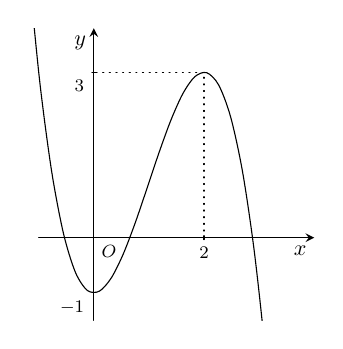
\begin{tikzpicture}[line join=round, line cap=round,>=stealth,scale=0.7]
			\tikzset{every node/.style={scale=0.8}}
			\draw[->] (-1,0)--(4,0) node[below left] {$x$};
			\draw[->] (0,-1.5)--(0,3.8) node[below left] {$y$};
			\draw (0,0) node [below right] {\footnotesize $O$};
			\foreach \x in {2}
			\draw[thin] (\x,1pt)--(\x,-1pt) node [below ] {\footnotesize $\x$};
			\foreach \y in {-1,3}
			\draw[thin] (1pt,\y)--(-1pt,\y) node [below left] {\footnotesize $\y$};
			\begin{scope}
				\clip (-1.2,-1.5) rectangle (4,3.8);
				\draw[domain=-1.2:4,smooth,variable=\x]
				plot (\x,{-1*(\x)^3+3*(\x)^2+0*(\x)+-1});
			\end{scope}
			\draw[dotted](2,0)|-(0,3);
		\end{tikzpicture}
	\end{center}
	Điểm cực đại của hàm số $y = f(x)$ là
	\choice
	{$x = 0$}
	{\True $x = 2$}
	{$y = 3$}
	{$M(2;3)$}
	\loigiai{
		Dựa vào đồ thị ta có điểm cực đại của hàm số là $x = 2$.
	}
\end{ex}
\begin{ex}%[1D5N1-1]
	Cô Hải thống kê đường kính thân gỗ của một số cây xoan đào $6$ năm tuổi được trồng ở một lâm trường như sau:
	\begin{center}
		\renewcommand{\arraystretch}{1.5}
		\begin{tabular}{|c|c|c|c|c|c|c|}
			\hline
			Đường kính (cm) & $[40; 45)$ & $[45; 50)$ & $[50; 55)$ & $[55; 60)$ & $[60; 65)$ & $[65; 70)$ \\
			\hline
			Tần số & $5$ & $20$ & $18$ & $7$ & $3$ & $1$ \\
			\hline
		\end{tabular}
	\end{center}
	Khoảng biến thiên của mẫu số liệu ghép nhóm trên là
	\choice
	{\True $30$}
	{$25$}
	{$18$}
	{$5$}
	\loigiai{
		Khoảng biến thiên của mẫu số liệu ghép nhóm trên là $R = 70 - 40 = 30$.
	}
\end{ex}
\begin{ex}%[2D1N4-1]
	Đường tiệm cận đứng của đồ thị hàm số $y = \dfrac{2x+3}{x-1}$ là
	\choice
	{$x = 2$}
	{$y = 1$}
	{$y = 2$}
	{\True $x = 1$}
	\loigiai{
		Tập xác định $\mathscr{D}=\mathbb{R}\setminus\{1\}$.\\
		Ta có $\displaystyle \lim \limits_{x \rightarrow 1^+} y = \displaystyle \lim \limits_{x \rightarrow 1^+} \dfrac{2x+3}{x-1} = +\infty \Rightarrow x = 1$ là tiệm cận đứng của đồ thị hàm số.
	}
\end{ex}
\begin{ex}%[1D2H2-2]
	Một cấp số nhân có ba số hạng liên tiếp là $12$; $30$; $a$. Tính $2a$.
	\choice
	{$81$}
	{\True $150$}
	{$75$}
	{$56$}
	\loigiai{
		Công bội của cấp số nhân $q = \dfrac{30}{12} = \dfrac{5}{2}$. \\
		Do đó, $a = 30\cdot\dfrac{5}{2} = 75$. \\
		Vậy $2a = 150$.
	}
\end{ex}
\begin{ex}%[1D3V3-4]
	Cho hàm số $f(x) = \heva{&\dfrac{\sqrt{x+1}-2}{x-3} & \text{khi } x > 3 \\& mx+2 & \text{khi } x \leq 3}$. Tìm giá trị của tham số $m$ để hàm số $f(x)$ liên tục trên $\mathbb{R}$.
	\choice
	{$\dfrac{1}
		{12}$}
	{$-\dfrac{7}
		{4}$}
	{$\dfrac{1}{4}$}
	{\True $-\dfrac{7}{12}$}
	\loigiai{
		Ta thấy hàm số liên tục trên khoảng $(-\infty;3)$ và $(3;+\infty)$. \\
		Để hàm số liên tục trên $\mathbb{R}$ khi và chỉ khi hàm số liên tục tại $x = 3$. \\
		Ta có $f(3) = \displaystyle \lim \limits_{x \rightarrow 3^-} f(x) = \displaystyle \lim \limits_{x \rightarrow 3^-} (mx+2) = 3m+2$;\\
		Mà $\displaystyle \lim \limits_{x \rightarrow 3^+} f(x) = \displaystyle \lim \limits_{x \rightarrow 3^+} \dfrac{\sqrt{x+1}-2}{x-3} = \displaystyle \lim \limits_{x \rightarrow 3^+} \dfrac{(x-3)}{(x-3).(\sqrt{x+1}+2)} = \displaystyle \lim \limits_{x \rightarrow 3^+} \dfrac{1}{\sqrt{x+1}+2} = \dfrac{1}{4}$. \\
		Do đó để hàm số liên tục tại $x = 3$ khi $f(3) = \displaystyle \lim \limits_{x \rightarrow 3^-} f(x) = \displaystyle \lim \limits_{x \rightarrow 3^-}f(x)$.\\
		Hay $3m+2 = \dfrac{1}{4} \Leftrightarrow 3m = -\dfrac{7}{4} \Leftrightarrow m=-\dfrac{7}{12}$.
	}
\end{ex}

\Closesolutionfile{ans}


\cauds
\Opensolutionfile{ans}[ans/ans-26-20-lientruongNgheAn-L2-DS]
\begin{ex}%[2D3V2-3]
	Khảo sát thời gian tập thể dục mỗi ngày (tính theo phút) của $32$ người thuộc hai câu lạc bộ: CLB Yoga và CLB Gym. Kết quả được thu thập và tổng hợp trong bảng tần số ghép nhóm dưới đây:
	\begin{center}
		\begin{tabular}{|c|c|c|c|c|c|}
			\hline
			Thời gian (phút) & [30; 50) & [50; 70) & [70; 90) & [90; 110) & [110; 130) \\
			\hline
			CLB Yoga	& 2 & 3 & 6 & 3 & 2 \\
			\hline
			CLB Gym	& 4 & 1 & 6 & 1 & 4 \\
			\hline
			Tổng số	& 6 & 4 & 12 & 4 & 6 \\
			\hline
		\end{tabular}
	\end{center}
	Xét tính đúng sai của các khẳng định sau.
	\choiceTF
	{\True Khoảng biến thiên của mẫu số liệu ghép nhóm cho cả $32$ người là $R=100$ (phút)}
	{Khoảng tứ phân vị của mẫu số liệu ghép nhóm cho cả $32$ người là $60$(phút)}
	{\True Mức độ tập luyện của những người ở CLB Yoga ổn định (đồng đều) hơn CLB Gym}
	{\True Chọn ngẫu nhiên $4$ người từ $32$ người trên. Xác suất để trong $4$ người được chọn có cả hai CLB Yoga, Gym và có đúng 2 người tập thể dục từ 110 phút trở lên là $\dfrac{4388}{35960}$}
	\loigiai{
		\begin{itemchoice}
			\itemch Khoảng biến thiên cho tổng $32$ người là $130-30=100$ (phút).
			\itemch Ta có:
			$Q_{1}=50+\dfrac{\dfrac{32}{4}+6}{4}\cdot (70-50)=60$.\\
			$Q_{3}=90+\dfrac{\dfrac{3}{4}\cdot 32-22}{4}\cdot (110-90)=100$.\\
			Nên khoảng tứ phân vị là $100-60=40$ (phút).
			\itemch Trung bình thời gian tập luyện của CLB Yoga là\\
			$\overline{x}_1=\dfrac{1}{16}(2\cdot 40+3\cdot 60+6\cdot 80+3\cdot 100+2\cdot 120)=80$.\\
			Phương sai của mẫu dữ liệu của CLB Yoga:\\
			$s_{1}^2=\dfrac{1}{16}[2\cdot 40^2+3\cdot 60^2+6\cdot 80^2+ 3\cdot 100^2+2\cdot 120^2 ]-{80}^2=550$.\\
			Trung bình thời gian tập luyện của CLB Gym\\
			$\overline{x}_2=\dfrac{1}{16}(4\cdot 40+1\cdot 60+6\cdot 80+1\cdot 100+4\cdot 120)=80$.\\
			Phương sai của mẫu dữ liệu của CLB Gym:\\
			$s_{2}^2=\dfrac{1}{16}(4\cdot 40^2+1\cdot 60^2+6\cdot 80^2+1\cdot 100^2+4\cdot 120^2)-80^2=850$.\\
			Vì $s_{2}^2> s_{1}^2$ nên mức độ tập luyện của những người ở CLB Yoga ổn định (đồng đều) hơn CLB Gym.
			\itemch Không gian mẫu $n(\Omega)=\mathrm{C}_{32}^4=35\,960$.\\
			Số người tập luyện $110$ phút trở lên có: 2 người ở CLB Yoga và 4 người ở CLB Gym.\\
			TH1: Chọn 4 người sao cho có cả CLB Gym, CLB yoga và có đúng 2 người tập luyện $110$ phút trở lên có cả 2 người ở CLB Yoga có\\
			$\mathrm{C}_{2}^2\cdot (\mathrm{C}_{14}^{1} \cdot \mathrm{C}_{12}^{1}+\mathrm{C}_{12}^2)=234$ (cách chọn).\\
			TH2: Chọn 4 người sao cho có cả CLB Gym, CLB yoga và có đúng 2 người tập luyện $110$ phút trở lên có cả 2 người ở CLB Gym có\\
			$\mathrm{C}_{4}^2(\mathrm{C}_{14}^{1}\cdot \mathrm{C}_{12}^{1}+\mathrm{C}_{14}^2)=1554$ (cách chọn).\\
			TH3: Chọn 4 người sao cho có cả CLB Gym, CLB yoga và có đúng 2 người tập luyện $110$ phút trở lên có 1 người ở CLB Gym và người còn lại ở CLB Yoga có\\ $\mathrm{C}_{4}^{1}\mathrm{C}_{2}^{1}(\mathrm{C}_{12}^{1}\cdot \mathrm{C}_{14}^{1}+\mathrm{C}_{12}^2+\mathrm{C}_{14}^2)=2600$.\\
			Vậy xác suất để trong 4 người được chọn có cả hai CLB Yoga, Gym và có đúng 2 người tập thể dục từ 110 phút trở lên là\\ $P=\dfrac{234+1554+2600}{35960}=\dfrac{4388}{35960}$.
		\end{itemchoice}
	}
\end{ex}
\begin{ex}%[2D1H3-2]
	Cho hàm số $y=\dfrac{-x^2+5x-7}{x-2}$ có đồ thị $(C)$. Xét tính đúng sai của các khẳng định sau.
	\choiceTF
	{\True Hàm số nghịch biến trên $(-\infty;1)$}
	{\True Khoảng cách giữa hai điểm cực trị của đồ thị $(C)$ bằng $2\sqrt{5}$}
	{Đồ thị hàm số có tiệm cận xiên là $y=-x-3$}
	{\True Giá trị nhỏ nhất của hàm số trên $\left[-2026;\dfrac{3}{2}\right]$ bằng $3$}
	\loigiai{
		$y=\dfrac{-x^2+5x-7}{x-2}=\dfrac{-(x-2)(x-3)-1}{x-2}=-x+3-\dfrac{1}{x-2}$.\\
		$y'=-1+\dfrac{1}{(x-2)^2}$;
		$y'=0\Leftrightarrow (x-2)^2=1\Leftrightarrow \hoac{
			& x=3\\
			& x=1.}$\\
		Bảng biến thiên
		\begin{center}
			
\begin{tikzpicture}
				\tikzset{double style/.append style={double distance=1.5pt}}
				\tkzTabInit[nocadre=false,lgt=1.2,espcl=2.5,deltacl=0.6]
				{$x$ /0.6,$y'$ /0.6,$y$ /2}
				{$-\infty$,$1$,$2$,$3$,$+\infty$}
				\tkzTabLine{,-,$0$,+,d,+,$0$,-,}
				\tkzTabVar{+/$+\infty$,-/$3$,+D-/$+\infty$/$-\infty$,+/$-1$,-/$-\infty$}
			\end{tikzpicture}
		\end{center}
		\begin{itemchoice}
			\itemch Hàm số nghịch biến trên $(-\infty;1)$ và $(3;+\infty)$.
			\itemch Từ bảng biến ta có hai điểm cực trị của đồ thị hàm số là $A(1;3)$; $B(3;-1)$\\
			$\Rightarrow AB=\sqrt{4+16}=2\sqrt{5}$.
			\itemch Ta có $\lim\limits_{x\to +\infty }[f(x)-(-x+3)]=\lim\limits_{x\to +\infty}\dfrac{-3}{x-2}=0$.\\
			Suy ra đường thẳng $y=-x+3$ là tiệm cận xiên của đồ thị hàm số.
			\itemch Đặt $M=\left[-2026;\dfrac{3}{2}\right]$.\\
			Ta có $y(1)=3$; $y(-2026)=\dfrac{4114813}{2028}$; $y\left(\dfrac{3}{2}\right)=\dfrac{7}{2}$.\\
			Suy ra $\min\limits_{M}y=3$.
		\end{itemchoice}
	}
\end{ex}
\begin{ex}%[2D1V5-8]
	Một hãng công nghệ dự định tung ra thị trường một loại tai nghe không dây mới. Chi phí sản xuất mỗi chiếc tai nghe là $500$ nghìn đồng với giá bán ra niêm yết là $1{,}2$ triệu đồng. Bộ phận bán hàng ước tính rằng, số lượng tai nghe bán được $n(x)$ phụ thuộc vào chi phí quảng cáo $x$ (đơn vị: triệu đồng) theo công thức $n(x)=A+30\ln (1+x)$. Biết rằng nếu chi $\mathrm{e}^3-1$ triệu đồng cho quảng cáo thì bán được $190$ sản phẩm. Xét tính đúng sai của các khẳng định sau.
	\choiceTF
	{\True $A=100$}
	{Hàm lợi nhuận của hãng (tính theo triệu đồng) là $L(x)=70+21\ln(x+1)-2x$}
	{Khi chi phí quảng cáo đang ở mức $6$ triệu đồng thì lợi nhuận đạt $99$ triệu đồng (kết quả làm tròn đến hàng đơn vị)}
	{Để đạt lợi nhuận lớn nhất thì số tiền chi cho quảng cáo là $19{,}766$ triệu đồng (kết quả làm tròn đến hàng phần nghìn)}
	\loigiai{
		\begin{itemchoice}
			\itemch Ta có $A+30 \ln \left(1+{\mathrm{e}^3}-1 \right)=190 \Leftrightarrow A+90=190 \Leftrightarrow A=100$.
			\itemch Ta có hàm lợi nhuận \\
			$L(x)=1{,}2\cdot n(x)-0{,}5\cdot n(x)-x=0{,}7(100+30\ln (1+x))-x =70+21\ln(1+x)-x$.
			\itemch Khi $x=6$ ta có $L(6)=70+21\ln(1+6)-6\approx 105$ (triệu đồng).
			\itemch Ta khảo sát hàm số $L(x)=70+21\ln(1+x)-x$.\\
			Ta có $L'(x)=\dfrac{21}{1+x}-1$\\
			$L'(x)=0\Leftrightarrow x=20$.\\
			Ta có bảng biến thiên
			\begin{center}
				
\begin{tikzpicture}
					\tkzTabInit[nocadre=false,lgt=1.5,espcl=2.5,deltacl=0.6]
					{$x$ /0.6,$L'(x)$ /0.6,$L(x)$ /2}
					{$0$,$20$,$+\infty$}
					\tkzTabLine{,+,$0$,-,}
					\tkzTabVar{-/$-\infty$, +/$ $,-/$-\infty$}
				\end{tikzpicture}
			\end{center}
			Vậy lợi nhuận đạt lớn nhất khi số tiền chi cho quảng cáo là $20$ triệu đồng.
		\end{itemchoice}
	}
\end{ex}
\begin{ex}%[2H2V2-6]
	\immini[thm]{Bạn Mạnh rất yêu thích tập Gym và bạn thường thực hiện bài tập ép ngực với máy tập cáp chéo có tên Tiếng Anh là "Cable Crossover". Thiết lập hệ trục tọa độ $Oxyz$ với đơn vị trên mỗi trục là mét có gốc tọa độ $O(0;0;0)$ nằm trên sàn ngay chính giữa hai trụ của máy tập, các trục $Ox, Oy, Oz$ được chọn như hình vẽ minh họa. Các ròng rọc cùa hai dây cáp được gắn tại các điểm $A(-1{,}3;0;1{,}9)$ và $B(1{,}3;0;1{,}9)$. Khi tập thì Mạnh kéo và giữ hai tay cầm tại điểm $D(0;0{,}7;1{,}2)$ và tại đó hai tay sẽ chịu tác dụng của hai lực căng $\vec{T}_{1}$ và $\vec{T}_{2}$. Biết rằng mức tạ được cài đặt sao cho độ lớn lực căng trên mỗi sợi dây cáp đều là $320$ N (kết quả tính được ở các ý đều làm tròn đến hàng phần trăm). Xét tính đúng sai của các khẳng định sau.
	}
	{\begin{tikzpicture}[scale=0.67,line cap=round, line join=round,>=stealth]
			\draw[->,thick] (0,-0.54) coordinate (O)--++(90:6) node[left] {$z$};
			\draw[->,thick] (O)--++(5:5) node[below] {$x$};
			\draw[->,thick] (O)--++(-35:3) node[right] {$y$};
			\draw[thick] (O)--++(-175:5);
			\draw[fill=black] (O) circle (2pt) node[below left] {$O$};
			%Đầu
			\def\e{(0.65,4.23)..controls++(259:0.3) and++(245:0.2)..(1.05,3.94)..controls++(-21:0.13) and++(243:0.05)..(1.23,4.01)}
			\draw[fill=brown!20] (0.72,4.39)..controls++(297:0.09) and++(71:0.06)..\e--cycle;
			\def\a{(1.4,4.74)..controls++(257:0.26) and++(69:0.39)..(1,4.59)..controls++(233:0.42) and++(38:0.22)..(0.73,4.54)};
			\draw[fill=black] (0.73,4.53)..controls++(89:0.75) and++(97:0.22)..\a;
			\draw[fill=pink!30] (1.4,4.74)..controls++(257:0.26) and++(69:0.39)..(1,4.59)..controls++(233:0.42) and++(38:0.22)..(0.73,4.54)..controls++(263:0.41) and++(77:0.29)..(0.82,4.19)..controls++(321:0.05) and++(249:0.52)..(1.29,4.13)..controls++(46:0.21) and++(214:0.13)..(1.43,4.4)..controls++(89:0.13) and++(324:0.09)..(1.4,4.74);
			\draw (1.23,4.42)..controls++(17:0.06) and++(61:0.04)..(1.1,4.47) (1.23,4.17)--(1.29,4.19)..controls++(92:0.2) and++(176:0.14)..(1.43,4.4) (1.11,4.12)..controls++(-35:0.03) and++(187:0.04)..(1.23,4.09);
			\draw[fill=black] (1.15,4.4) circle (1pt) (1.34,4.36) circle (1pt);
			%Áo
			\draw[fill=orange] (-0.13,3.6)..controls++(91:0.63) and++(207:0.09)..\e..controls++(332:0.36) and++(122:0.27)..(1.53,3.35)..controls++(158:0.26) and++(25:0.15)..(1.1,3.23)..controls++(245:0.42) and++(67:0.8)..(0.65,2.46)..controls++(231:0.42) and++(307:0.65)..(-0.52,2.71)..controls++(46:0.45) and++(235:0.27)..(-0.13,3.6);
			%Chân trái
			\draw[fill=brown!30] (-0.89,1.61)..controls++(239:0.39) and++(45:0.46)..(-1.24,1.06)..controls++(233:0.21) and++(73:0.61)..(-1.45,0.35)..controls++(244:0.26) and++(61:0.07)..(-1.24,0.21)..controls++(75:0.48) and++(256:0.31)..(-0.77,0.96)..controls++(64:0.24) and++(262:0.16)..(-0.41,1.44)--cycle;
			%Trân phải
			\draw[fill=brown!30] (0.24,1.62)..controls++(292:0.42) and++(58:0.5)..(0.43,0.84)..controls++(240:0.32) and++(73:0.64)..(0.38,-0.1)..controls++(276:0.15) and++(233:0.19)..(0.64,-0.18)..controls++(81:0.8) and++(279:0.46)..(0.88,1.03)..controls++(45:0.17) and++(264:0.32)..(0.9,1.77)--cycle;
			%Tay
			\draw[fill=brown!20] (0.56,3.25)..controls++(151:0.16) and++(53:0.22)..(0.09,3.13)..controls++(298:0.73) and++(151:1.38)..(1.19,2.2)..controls++(291:0.15) and++(237:0.42)..(1.69,2.21)..controls++(90:1.09) and++(278:0.41)..(1.52,3.34)..controls++(144:0.09) and++(46:0.26)..(1.11,3.22)..controls++(282:0.38) and++(103:0.64)..(1.43,2.47)..controls++(206:0.35) and++(322:0.24)..(0.8,2.8)..controls++(146:0.38) and++(286:0.49)..(0.56,3.25);
			%Quần
			\draw[fill=teal!80!black] (-0.95,1.63)..controls++(52:0.34) and++(222:0.34)..(-0.52,2.71)..controls++(307:0.65) and++(231:0.42)..(0.65,2.46)..controls++(268:0.24)
			and++(91:0.55)..(0.91,1.61)..controls++(144:0.45) and++(270:0)..(0.19,1.46)..controls++(270:0) and++(298:0.16)..(0.02,1.83)..controls++(235:0.21) and++(70:0.23)..(-0.25,1.42)..controls++(194:0.26) and++(318:0.31)..(-0.95,1.63);
			\draw[fill=teal!80!black] (0.28,1.56)..controls++(211:0.03) and++(53:0.04)..(0.19,1.46)--(0.34,1.46)--cycle;
			%đường phụ
			\draw (-0.11,3.62)..controls++(272:0.12) and++(113:0.27)..(0.08,3.13);
			\draw (0.32,3.88)..controls++(-14:0.14) and++(78:0.18)..(0.53,3.42)..controls++(289:0.04) and++(59:0.02)..(0.56,3.27);
			\draw (0.6,3.72)..controls++(269:0.12) and++(31:0.05)..(0.53,3.42)..controls++(140:0.04) and++(-15:0.14)..(0.29,3.57);
			\draw (1.22,3.74)..controls++(289:0.16) and++(52:0.14)..(1.09,3.21) (1.31,3.6)..controls++(250:0.12) and++(41:0.1)..(1.17,3.38) (-0.28,2.78)..controls++(-45:0.4) and++(182:0.33)..(0.41,2.47) (1.62,2.46)..controls++(-29:0.16) and++(-34:0.1)..(1.47,2.38);
			\draw (1.49,2.29) -- (1.56,2.25) -- (1.66,2.28) -- (1.71,2.32) (1.46,2.20) -- (1.53,2.18) -- (1.61,2.18) -- (1.67,2.21) -- (1.68,2.27) (1.43,2.14) -- (1.50,2.10) -- (1.59,2.11) -- (1.62,2.13) -- (1.61,2.18) (1.38,2.08) -- (1.42,2.06) -- (1.47,2.04) -- (1.53,2.05) -- (1.56,2.08) (1.49,2.29) -- (1.46,2.25) -- (1.46,2.20) -- (1.43,2.19) -- (1.43,2.14) -- (1.39,2.13) -- (1.38,2.08);
			%Tay nắm kéo
			\draw[fill=blue] (1.31,2.08)..controls++(256:0.11) and++(242:0.09)..(1.46,2.03)..controls++(151:0.14) and++(14:0.12)..(1.31,2.08) (1.45,2.38)..controls++(66:0.25) and++(111:0.12)..(1.64,2.51)..controls++(233:0.22) and++(-15:0.2)..(1.45,2.38);
			\draw (-0.3,1.68)..controls++(19:0.27) and++(290:0.09)..(0.24,2.16) (0.03,1.87)..controls++(16:0.1) and++(174:0.15)..(0.41,1.94) (-0.01,1.83)..controls++(46:0.26) and++(226:0.14)..(0.38,2.13) (0.07,1.87)..controls++(-10:0.15) and++(156:0.19)..(0.5,1.73);
			%Giay
			\draw[fill=teal] (-1.45,0.36)..controls++(226:0.22) and++(122:0.22)..(-1.57,-0.11)..controls++(-36:0.06) and++(179:0.52)..(-1.24,-0.46)..controls++(5:0.33) and++(251:0.08)..(-1.19,-0.07)..controls++(94:0.18) and++(288:0.07)..(-1.22,0.26)..controls++(198:0.05) and++(-12:0.12)..(-1.32,0.23)..controls++(165:0.11) and++(256:0.34)..(-1.45,0.36);
			\draw[fill=blue!30] (-1.58,0.19)..controls++(286:0.35) and++(166:0.32)..(-1.32,-0.42)..controls++(87:0.07) and++(97:0.05)..(-1.16,-0.39)..controls++(49:0.03) and++(276:0.08)..(-1.11,-0.27)..controls++(296:0.3) and++(271:0.27)..(-1.59,-0.26)..controls++(75:0.32) and++(244:0.34)..(-1.58,0.19);
			\draw[fill=red] (-1.42,0.08)..controls++(108:0.1) and++(179:0.13)..(-1.34,0.22)..controls++(2:0.13) and++(92:0.1)..(-1.25,0.09);
			\draw (-1.42,0.05) -- (-1.25,0.01) (-1.26,0.06) -- (-1.4,0.0) -- (-1.25,-0.04) -- (-1.42,0.05) (-1.25,-0.04) -- (-1.38,-0.1) -- (-1.24,-0.12) -- (-1.4,0.0) (-1.24,-0.12) -- (-1.39,-0.18) -- (-1.23,-0.17) -- (-1.38,-0.1);
			%giầy
			\draw[fill=teal] (0.39,-0.09)..controls++(185:0.09) and++(56:0.12)..(0.23,-0.42)..controls++(236:0.08) and++(180:0.25)..(0.51,-0.58)..controls++(321:0.23) and++(283:0.26)..(1.07,-0.56)..controls++(140:0.19) and++(262:0.17)..(0.7,-0.08)..controls++(131:0.09) and++(145:0.12)..(0.51,-0.17)..controls++(157:0.05) and++(258:0.16)..(0.39,-0.09);
			\draw[fill=blue!30] (0.28,-0.32)..controls++(238:0.08) and++(179:0.42)..(0.5,-0.59)..controls++(-35:0.35) and++(289:0.14)..(1.08,-0.59)..controls++(183:0.21) and++(4:0.12)..(0.89,-0.65)..controls++(171:0.24) and++(-23:0.07)..(0.53,-0.45)..controls++(174:0.12) and++(272:0.13)..(0.28,-0.32);
			\draw (0.33,-0.19)..controls++(270:0.2) and++(146:0.39)..(0.95,-0.6) ;
			\draw[fill=red] (0.51,-0.19)..controls++(301:0.2) and++(172:0.18)..(0.71,-0.19) ..controls++(89:0.17) and++(18:0.09)..(0.56,-0.07)..controls++(197:0.09) and++(126:0.09)..(0.51,-0.19);
			\draw (0.63,-0.3) -- (0.8,-0.32) -- (0.7,-0.37) -- (0.84,-0.37) -- (0.76,-0.43) -- (0.87,-0.43) -- (0.7,-0.37) (0.81,-0.37) -- (0.63,-0.3) (-0.87,0.94)..controls++(41:0.06) and++(235:0.07)..(-0.73,1.04) (0.54,1.09)..controls++(277:0.06) and++(79:0.06)..(0.57,0.93);
			%Khung
			\draw[fill=gray] (-4.39, -0.65) -- (-4.39, -0.42) -- (-4.24, -0.46) -- (-3.75, 0.23) -- (-3.74, 5.93) -- (-3.8, 5.97) -- (-3.8, 6.6) -- (-3.55, 6.64) -- (-3.56, 5.99) -- (-3.6, 5.96) -- (-3.61, 0.17) -- (-3.09, -0.78) -- (-3.0, -0.8) -- (-3.01, -1.05) -- cycle;
			\draw[fill=orange] (-3.0, -0.8) -- (-3.02, -1.12) -- (-2.76, -1.2) -- (-2.4, -1.13) -- (-2.41, -0.83) -- (-2.68, -0.74) -- cycle;
			\draw (-3.0, -0.8) -- (-2.75, -0.87) -- (-2.76, -1.2) (-2.75, -0.87) -- (-2.41, -0.83);
			\draw[fill=orange] (-4.31, -0.67) -- (-4.39, -0.69) -- (-4.62, -0.63) -- (-4.63, -0.35) -- (-4.32, -0.3) -- (-4.17, -0.36) -- (-4.2, -0.4) -- (-4.39, -0.42) -- (-4.39, -0.65) -- cycle;
			\draw[fill=gray!30] (-4.39, -0.42) -- (-4.24, -0.46) -- (-4.2, -0.4) -- cycle;
			\draw[fill=gray!30] (-3.0, -0.8) -- (-2.74, -0.76) -- (-2.91, -0.72) -- (-3.42, 0.17) -- (-3.41, 5.97) -- (-3.6, 5.96) -- (-3.61, 0.17) -- (-3.09, -0.78) -- cycle;
			\draw[fill=orange] (-3.55, 6.64) -- (-3.08, 6.6) -- (-3.08, 6.3) -- (-3.35, 6.1) -- (-3.36, 5.97) -- (-3.6, 5.96) -- (-3.56, 5.99) -- cycle;
			\draw[fill=gray!30] (-3.1, 6.56) -- (3.05, 6.14) -- (3.05, 5.96) -- (-3.1, 6.3) -- cycle;
			\draw[fill=orange] (2.9, 6.15) -- (2.9, 6.27) -- (3.45, 6.25) -- (3.45, 5.66) -- (3.3, 5.66) -- (3.1, 5.92) -- (3.05, 5.96) -- (3.05, 6.14) -- cycle;
			\draw[fill=gray] (3.3, 5.66) -- (3.1, 5.66) -- (2.9, 5.94) -- (2.9, 5.96) -- (3.05, 5.96) -- (3.1, 5.92) -- cycle;
			\draw[fill=gray!30] (3.45, 5.66) -- (3.45, 0.66) -- (3.95, -0.04) -- (4.15, -0.08) -- (3.95, -0.13) -- (3.8, -0.11) -- (3.3, 0.66) -- (3.3, 5.66) -- cycle;
			\draw[fill=gray] (3.15, 5.66) -- (3.3, 5.66) -- (3.3, 0.66) -- (3.8, -0.11) -- (3.95, -0.13) -- (3.95, -0.35) -- (2.45, -0.07) -- (2.45, 0.12) -- (2.65, 0.1) -- (3.15, 0.66) -- cycle;
			\draw[fill=orange] (3.95, -0.13) -- (4.2, -0.07) -- (4.5, -0.12) -- (4.5, -0.38) -- (4.2, -0.43) -- (3.95, -0.39) -- cycle;
			\draw[fill=orange] (2.45, 0.12) -- (2.7, 0.17) -- (2.7, 0.19) -- (2.5, 0.24) -- (2.2, 0.19) -- (2.2, -0.05) -- (2.45, -0.1) -- (2.5, -0.08) -- (2.45, -0.07) -- cycle;
			\draw (-3.09, -0.78) -- (-2.91, -0.72)
			(-4.39, -0.42) -- (-4.63, -0.35)
			(-3.61, 0.17) -- (-3.42, 0.17)
			(2.2, 0.19) -- (2.45, 0.12)
			(3.95, -0.13) -- (4.2, -0.17) -- (4.48, -0.12)
			(4.2, -0.17) -- (4.2, -0.43)
			(3.82, -0.11) -- (3.95, -0.04)
			(3.28, 0.66) -- (3.44, 0.66);
			\draw[fill=blue!60] (2.91,5.94)..controls++(232:0.18) and++(256:0.3)..(3.17,5.82)..controls++(121:0.2) and++(0:0.12)..(2.91,5.94);
			\draw[fill=blue!60] (-3.32,6.1)..controls++(292:0.32) and++(331:0.34)..(-3.1,6.27)--cycle;
			\draw[fill=gray] (-3.34,6.42) circle (2pt) (3.3,6.06) circle (2pt);
			\draw[line width=1pt,black] (-3.04,6.02) coordinate (A)--(1.43,2.24) coordinate (D) (1.63,2.55)coordinate (C)--(3.01,5.71) coordinate (B);
			\draw[->, red, line width=2pt] ($(D)!0.5!(A)$)--($(D)!0.7!(A)$) node[above] {$\overrightarrow{T_1}$};
			\draw[->, red, line width=2pt] ($(C)!0.5!(B)$)--($(C)!0.7!(B)$) node[above] {$\overrightarrow{T_2}$};
		\end{tikzpicture}
	}
	\choiceTF
	{\True Chiều dài đoạn dây cáp tính từ ròng rọc $A$ đến tay cầm $D$ bằng $1{,}63$ m}
	{\True Vectơ hợp lực tác dựng lên tay Mạnh có phương không song song với trục $Oz$}
	{\True Để giữ yên hai tay tại vị trí $D$ thì Mạnh phải tác dụng một lực giữ có độ lớn bằng $387{,}74$ N}
	{Để tối ưu hóa nhóm cơ ngực, huấn luyện viên yêu cầu Mạnh điều chinh vị trí giữ tay (thay đổi tung độ $y$ của điểm $D$) sao cho góc tạo bởi hai dây cáp tại $D$ đúng bằng $90^{\circ}$. Biết cao độ của tay vẫn giữ nguyên ở $z_{D}=1{,}2$ m thì khi đó Mạnh cần giữ tay cầm ở vị trí sao cho $y_{D}=0{,}99$ m}
	\loigiai{
		\begin{itemchoice}
			\itemch $\overrightarrow{DA}=(-1{,}3;-0{,}7; 0{,}7)\Rightarrow DA\approx 1{,}63$ m.
			\itemch Ta có:
			$\overrightarrow{DB}=(1{,}3;-0{,}7;0{,}7)$; 		$\overrightarrow{T}_{1}=k\overrightarrow{DA}$ và $\overrightarrow{T}_{2}=k\overrightarrow{DB}$ (với $k>0$)\\
			Vectơ hợp lực tác dụng lên tay Mạnh:\\
			$\overrightarrow{T}_{1}+\overrightarrow{T}_{2}=k(\overrightarrow{DA}+\overrightarrow{DB})=(0;-1{,}4k; 1{,}4k)$\\
			$\Rightarrow \overrightarrow{T}_{1}+\overrightarrow{T}_{2}$ không cùng phương $\vec{k}=(0;0;1)$.
			\itemch Lực giữ tay Mạnh có độ lớn bằng\\
			$|\overrightarrow{T}_{1}+\overrightarrow{T}_{2}|=k|\overrightarrow{DA}+\overrightarrow{DB}|=k\sqrt{0^2+(-1{,}4)^2+1{,}4^2}=1{,}4\cdot k\cdot \sqrt{2}$.\\
			Với $k=\dfrac{|\overrightarrow{T}_{1}|}{|\overrightarrow{DA}|}=\dfrac{320}{\sqrt{1{,}3^2+0{,}7^2+0{,}7^2}}=\dfrac{320}{\sqrt{2{,}67}}$\\
			$\Rightarrow |\overrightarrow{T}_{1}+\overrightarrow{T}_{2}|=1{,}4\cdot \sqrt{2}\cdot \dfrac{320}{\sqrt{2{,}67}}\approx 387{,}74$.
			\itemch $D(0;y_{D};1,2)$
			$\overrightarrow{DA}=(-1{,}3;-y_{D}; 0{,}7)$, $\overrightarrow{DB}=(1{,}3;-y_{D}; 0{,}7)$\\
			$\overrightarrow{DA}\cdot \overrightarrow{DB}=0 \Leftrightarrow -1+{3}^2+y_{D}^2+{0{,}7}^2=0 \Rightarrow y_{D} \approx 1{,}1$.
		\end{itemchoice}
} \end{ex}
\Closesolutionfile{ans}

\caukq
\Opensolutionfile{ans}[ans/ans-26-20-lientruongNgheAn-L2-KQ]
%-----Câu 1
\begin{ex}%[0D0C2-5]
	Một hộp đựng $25$ lá thăm khác nhau được đánh số từ $1$ đến $25$. Chọn ngẫu nhiên đồng thời $4$ lá thăm ở hộp. Tính xác suất để trong $4$ lá thăm được chọn có ít nhất $2$ lá thăm là số nguyên tố và tổng của $4$ số đó là một số chẵn (làm tròn đến hàng phần trăm).
	\shortans{0,23}
	\loigiai{
		Gọi $A$ là biến cố \lq\lq trong 4 lá thăm được chọn có ít nhất 2 lá thăm là số nguyên tố và tổng của 4 số đó là một số chẵn\rq\rq.\\
		$n(\Omega)=\mathrm{C}_{25}^4=12\,650$.\\
		Trong $25$ lá thăm có $1$ số chẵn là số nguyên tố, $8$ số lẻ là số nguyên tố, $11$ số chẵn không phải số nguyên tố  và $5$ số lẻ không phải nguyên tố.\\
		Để trong $4$ lá thăm được chọn có ít nhất $2$ lá thăm là số nguyên tố và tổng của $4$ số đó là một số chẵn ta có các trường hợp sau:
		\begin{itemize}
			\item \textbf{TH1:} $2$ số lẻ là số nguyên tố, $2$ số lẻ không là số nguyên tố, có $\mathrm{C}_8^2 \cdot \mathrm{C}_5^2=280$ cách chọn.
			\item \textbf{TH2:} $2$ số lẻ là số nguyên tố, $2$ số chẵn không là số nguyên tố, có $\mathrm{C}_8^2 \cdot \mathrm{C}_{11}^2=1\,540$ cách chọn.
			\item \textbf{TH3:} $1$ số lẻ là số nguyên tố, $1$ số chẵn là số nguyên tố, $1$ số chẵn không là số nguyên tố và $1$ số lẻ không là số nguyên tố có $\mathrm{C}_8^2 \cdot \mathrm{C}_1^1 \cdot \mathrm{C}_{11}^1 \cdot \mathrm{C}_5^2=440$ cách chọn.
			\item \textbf{TH4:} $3$ số lẻ là số nguyên tố, $1$ số lẻ không là số nguyên tố, có  $\mathrm{C}_8^3 \cdot \mathrm{C}_5^1=280$ cách chọn.
			\item \textbf{TH5:} $2$ số lẻ là số nguyên tố, $1$ số chẵn là số nguyên tố, $1$ số chẵn không là số nguyên tố, có  $\mathrm{C}_8^2 \cdot \mathrm{C}_1^1 \cdot \mathrm{C}_{11}^1=308$ cách chọn.
			\item \textbf{TH6:} $4$ số lẻ là số nguyên tố, có  $\mathrm{C}_8^4=70$ cách chọn.
		\end{itemize}
		Vậy $n(A)=1\,540+280+440+280+308+70=2\,918$.\\
		Vậy $\mathrm{P}(A)=\dfrac{n(A)}{n(\Omega)}=\dfrac{2\,918}{12\,650}\approx 0{,}23$.
	}
\end{ex}
%-----Câu 2
\begin{ex}%[2D1C5-8]
	Việt Nam đang triển khai dự án đường sắt tốc độ cao chặng Thành phố Hồ Chí Minh - Nha Trang với tổng chiều dài quãng đường là $375$ km. Tổng công ty đường sắt cần xác định vận tốc khai thác $v$ (km/h) cho đoàn tàu ($200 \le v \le 350$) để đạt lợi nhuận cao nhất cho mỗi chuyến tàu. Qua các số liệu tính toán kỹ thuật và khảo sát thị trường, ta có các thông tin sau: Chi phí điện năng tiêu thụ cho toàn bộ hành trình  được tính toán chính xác theo công thức $C_1(v)=15v^2$ (nghìn đồng). Chi phí vận hành cố định: bao gồm nhân sự, khẩu hao thiết bị và bảo trì đường ray tính cho mỗi giờ tàu chạy là $250$ triệu đồng/giờ. Số lượng khách mua về cho mỗi chuyến tàu phụ thuộc vào vận tốc $v$ theo hàm số $N(v)=4v$ (khách). Giá vé bình quân cố định cho toàn chặng là $1\,500\,000$ đồng/khách. Xác định vận tốc khai thác $v$ để lợi nhuận ròng của một chuyến tàu là lớn nhất (làm tròn kết quả đến hàng đơn vị).
	\shortans{250}
	\loigiai{
		Đổi đơn vị về triệu đồng, ta được $C_1(v)=15v^2$ (nghìn đồng) $=0{,}015v^2$ (triệu đồng).\\
		Giá vé bình quân cố định cho toàn chặng là $1\,500\,000$ đồng/khách hay $1{,}5$ triệu đồng/khách. Khi đó ta có
		\begin{itemize}
			\item Doanh thu của mỗi chuyến tàu là $$R(v)=1{,}5 \cdot 4v=6v \, \text{(triệu đồng)}.$$
			\item Chi phí mỗi chuyến tàu là $$C(v)=0{,}015v^2+\dfrac{375}{v} \cdot 250=0{,}015v^2+\dfrac{93\,750}{v} \, \text{(triệu đồng)}.$$
			\item Lợi nhuận ròng của chuyến tàu là $$f(v)=R(v)-C(v)=-0{,}015v^2+6v-\dfrac{93\,750}{v} \, \text{(triệu đồng)}$$  với $200 \le v \le 350$.
		\end{itemize}
		$f'(v)=-0{,}03v+6+\dfrac{93\,750}{v^2}=\dfrac{-0{,}03v^3+6v^2+93\,750}{v^2}$.\\
		$f'(v)=0 \Rightarrow v=250 \in [200;350]$.\\
		Ta có $f(200)=\dfrac{19\,125}{32}$; $f(250)=561$; $f(350)=\dfrac{12\,825}{49}$.\\
		Do đó $\max\limits_{[200;350]} f(v)=f(250)=561$.\\
		Vậy lợi nhuận ròng của một chuyến tàu lớn nhất khi $v=250$ (km/h).
	}
\end{ex}
%-----Câu 3
\begin{ex}%[2H2V2-6]
	Trong không gian $Oxyz$ (mỗi đơn vị trên trục tương ứng với $1$ km), tại thời điểm $8$ giờ sáng, hai máy bay $A$ và $B$ có vị trí và lộ trình chuyển động như sau
	\begin{itemize}
		\item Máy bay $A$: đang ở vị trí $M(0;0;9)$, bay thẳng theo hướng đến điểm $N(1\,200;0;9)$ với tốc độ hành trình $v_1=800$ km/h.
		\item Máy bay $B$: đang ở vị trí $P(103;-299;12)$ bay thẳng đều theo hướng đến điểm $Q(1\,003;601;12)$ với tốc độ hành trình $v_2=600\sqrt{2}$ km/h.
	\end{itemize}
	Hãy xác định khoảng cách ngắn nhất giữa hai máy bay $A$ và máy bay $B$ trong quá trình bay (làm tròn kết quả đến hàng phần trăm, đơn vị km).
	\shortans{4,36}
	\loigiai{
		Máy bay $A$ có vectơ $\overrightarrow{v}_1=k\overrightarrow{MN}$ ($k>0$).\\
		Ta có $\left|\overrightarrow{v}_1\right|=k_1 \left|\overrightarrow{MN}\right| \Leftrightarrow 800 = k_1\sqrt{1200^2+0^2+0^2} \Leftrightarrow k_1=\dfrac{2}{3}$.\\
		Khi đó $\overrightarrow{v}_1=\dfrac{2}{3}\overrightarrow{MN} \Rightarrow \overrightarrow{v}_1=(800;0;0)$.\\
		Sau $t$ (giờ) máy bay $A$ di chuyển đến $A_1(800t;0;9)$.\\
		Máy bay $B$ có vectơ $\overrightarrow{v}_2=k \overrightarrow{PQ}$ ($k>0$).\\
		Ta có $ \left|\overrightarrow{v}_2\right|=k_2 \left|\overrightarrow{PQ}\right| \Leftrightarrow 600\sqrt{2}=k_2\sqrt{900^2+900^2+0^2} \Leftrightarrow k_2=\dfrac{2}{3}$.\\
		Khi đó $ \overrightarrow{v}_2=\dfrac{2}{3} \overrightarrow{PQ} \Rightarrow \overrightarrow{v}_2=(600;600;0)$.\\
		Sau $t$ (giờ) máy bay $B$ di chuyển đến $B_1(103+600t;-299+600t;12)$.\\
		Xét $A_1B_1=\sqrt{(103-200t)^2+(-299+600t)^2+3^2}$.\\
		Khảo sát hàm số hoặc sử dụng Casio ta thấy $A_1B_1$ nhỏ nhất khi $t=\dfrac{1}{2}\Rightarrow A_1B_1=\sqrt{19} \approx 4{,}36$ là khoảng cách ngắn nhất của hai máy bay trong quá trình bay.
	}
\end{ex}
%-----Câu 4
\begin{ex}%[1H8V5-4]
	Cho hình chóp $S.ABCD$ có đáy $ABCD$ là hình chữ nhật, $AB=4$, $AD=8$, $SA$ vuông góc với đáy và $SA=4\sqrt{3}$. Tính khoảng cách giữa hai đường thẳng $SC$ và $BD$ (kết quả làm tròn đến hàng phần trăm).
	\shortans{2,49}
	\loigiai{
		\begin{center}
			\begin{tikzpicture}
				\def\a{5}
				\def\h{3.3}
				\path 	(0:0) coordinate (A)
				++(0:\a) coordinate (D)
				++(-135:\a/2) coordinate (C)
				($(A)+(C)-(D)$) coordinate (B)
				($(A)+(90:\h)$) coordinate (S)
				(intersection of A--C and B--D) coordinate (O)
				($(B)+(C)-(D)$) coordinate (E)
				($(C)!(A)!(E)$) coordinate (K)
				($(C)!(B)!(E)$) coordinate (F)
				($(S)!1/3!(K)$) coordinate (H)
				;
				\draw[dashed] 	(B)--(A)--(D)--(B)	(A)--(S) (B)-- (C) (E)--(B)--(S) (B)--(F) (A)--(K) (A)--(H);
				\draw	 (C)--(D)
				(C)--(S)	(D)--(S)
				(S)--(E)--(C) (S)--(K)
				;
				\foreach \x/\g in {A/135,B/180,C/-45,D/45,S/90,K/-90,E/-120,F/-85,H/0}
				\fill[black] 	(\x) circle (1.5pt)
				($(\g:3mm)+(\x)$) node {$\x$};
				\draw pic[draw,angle radius=4mm]{right angle=A--H--K};
				\draw pic[draw,angle radius=3mm]{right angle=B--F--C};
			\end{tikzpicture}
			\hspace{1cm}
			\begin{tikzpicture}
				\def\a{5}
				\def\h{2.5}
				\path 	(0:3) coordinate (B)
				++(0:\a) coordinate (C)
				++(90:\h) coordinate (D)
				++(0:-\a) coordinate (A)
				($(B)+(C)-(D)$) coordinate (E)
				($(C)!(A)!(E)$) coordinate (K)
				($(C)!(B)!(E)$) coordinate (F)
				;
				\draw	 (A)--(B)--(C)--(D)--(A) (B)--(D) (B)--(F) (A)--(K) (B)--(E)--(C)
				;
				\foreach \x/\g in {A/135,B/180,C/-45,D/45,E/180,K/-50,F/-50}
				\fill[black] 	(\x) circle (1.5pt)
				($(\g:3mm)+(\x)$) node {$\x$};
				\draw pic[draw,angle radius=3mm]{right angle=A--K--C};
				\draw pic[draw,angle radius=3mm]{right angle=B--F--C};
			\end{tikzpicture}
		\end{center}
		Kẻ $CE \parallel BC$ và $CE=BD$, dễ thấy $B$ là trung điểm $AE$.\\
		$BD \parallel (SEC) \Rightarrow \mathrm{d}(BD,SC)=\mathrm{d}(BD,(SEC))=\mathrm{d}(B,(SEC))=\dfrac{1}{2}\mathrm{d}(A,(SEC))$.\\
		Dựng $BF \perp EC$ tại $F$, $AK \perp EC$ tại $K \Rightarrow AK=2BF$.\\
		$\dfrac{1}{BF^2}=\dfrac{1}{BE^2}+\dfrac{1}{BC^2}=\dfrac{1}{4^2}+\dfrac{1}{8^2} \Rightarrow BF=\dfrac{8\sqrt{5}}{5} \Rightarrow AK=\dfrac{16\sqrt{5}}{5}$.\\
		Dựng $AH \perp SK$ tại $H \Rightarrow \mathrm{d}(A,(SEC))=AH$.\\
		$\dfrac{1}{AH^2}=\dfrac{1}{AK^2}+\dfrac{1}{SA^2}=\dfrac{1}{\left(\dfrac{16\sqrt{5}}{5}\right)^2}+\dfrac{1}{\left(4\sqrt{3}\right)^2} \Rightarrow AH=\dfrac{16\sqrt{93}}{31}$.\\
		Suy ra $\mathrm{d}(BD,SC)=\dfrac{1}{2}AH=\dfrac{8\sqrt{93}}{31} \approx 2{,}49$.
	}
\end{ex}
%-----Câu 5
\begin{ex}%[0D2V2-3]
	Một trang trại quy hoạch trồng bưởi da xanh và cam sành trên tổng diện tích tối đa là $10$ ha. Để trồng $1$ ha bưởi da xanh cần $20$ công lao động và $20$ triệu đồng tiền vốn. Để trồng $1$ ha cam sành cần $10$ công lao động và $20$ triệu đồng tiền vốn. Trang trại hiện có tối đa $160$ công lao động và nguồn vốn đầu tư không vượt quá $270$ triệu đồng. Lợi nhuận thu được ước tính là $30$ triệu/ha bưởi da xanh và $40$ triệu/ha cam sành. Hãy xác định mức lợi nhuận tối đa có thể đạt được (đơn vị triệu đồng).
	\shortans{370}
	\loigiai{
		Gọi diện tích để trồng bưởi da xanh là $x$ (ha, $x \ge 0$).\\
		Gọi diện tích để trồng cam sành là $y$ (ha, $y\ge 0$).\\
		Vì tổng diện tích tối đa để trồng bưởi da xanh và cam sành là $10$ ha nên ta có bất phương trình $x+y \le 10$.\\
		Vì trang trại có tối đa $160$ công lao động nên ta có $20x+10y \le 160$.\\
		Vì trang trại có vốn đầu tư không vượt quá $270$ triệu đồng nên ta có $20x+30y \le 270$.\\
		Từ các dữ kiện trên ta có hệ bất phương trình $\heva{&x \ge 0\\&y\ge 0\\&x+y \le 10\\&20x+10y \le 160\\&20x+30y \le 270.}$
		\begin{center}
			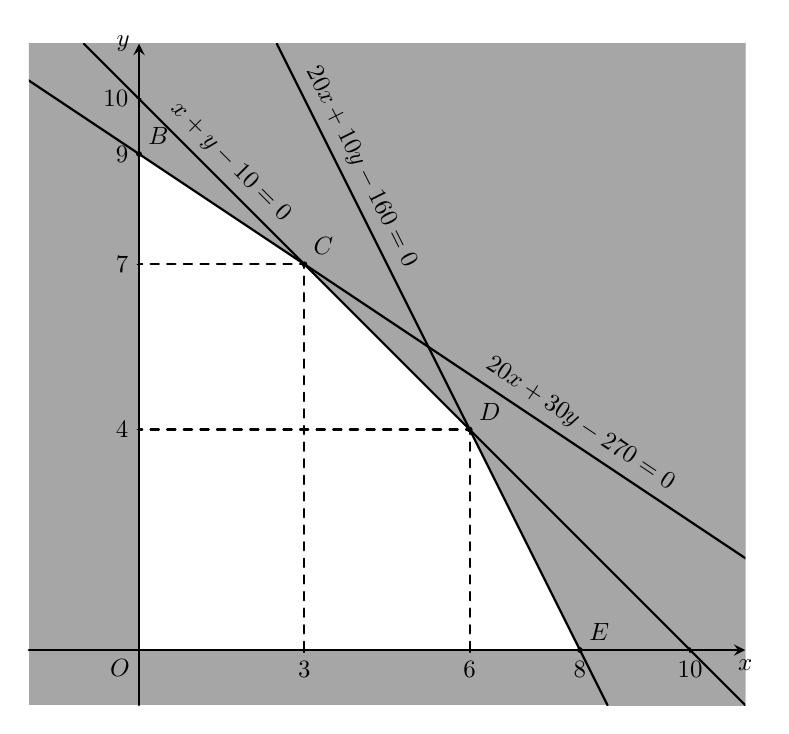
\begin{tikzpicture}[scale=0.7,line join=round, line cap=round,>=stealth,thick]
				\tikzset{every node/.style={scale=0.9}}
				\begin{scope}
					\clip (-2,-1) rectangle (11,11);
					\fill[black!35] (-3,13)--(12,13)--(12,-2)--cycle;
					\fill[black!35] (0,-1)--(-2,-1)--(-2,11)--(0,11)--cycle;
					\fill[black!35] (-2,0)--(-2,-1)--(11,-1)--(11,0)--cycle;
					\fill[black!35] (-3,22)--(12,22)--(12,-8)--cycle;
					\fill[black!35] (-4,11.67)--(16,11.67)--(16,-1.67)--cycle;
					\draw (-1,11)--(11,-1) node [pos=0.2, above, sloped] {$x+y-10=0$};
					\draw (2.5,11)--(8.5,-1) node [pos=0.2, above, sloped] {$20x+10y-160=0$};
					\draw (-3,11)--(15,-1) node [pos=0.6, above, sloped] {$20x+30y-270=0$};
				\end{scope}
				\draw[->] (-2,0)--(11,0) node[below]{$x$};
				\draw[->] (0,-1)--(0,11) node[left]{$y$};
				\draw (0,0) node[below left]{$O$};
				\foreach \x in {8,10,3,6}
				\draw (\x,1pt)--(\x,-1pt) node [below] {$\x$};
				\foreach \y in {9,10,4,7}
				\draw[thin] (1pt,\y)--(-1pt,\y) node [left] {$\y$};
				\draw[dashed] (6,0)--(6,4)--(0,4);
				\draw[dashed] (3,0)--(3,7)--(0,7);
				\fill 	(0,9) circle (1.5pt) node[above right]{$B$}
				(3,7) circle (1.5pt) node[above right]{$C$}
				(6,4) circle (1.5pt) node[above right]{$D$}
				(8,0) circle (1.5pt) node[above right]{$E$}
				;
			\end{tikzpicture}
		\end{center}
		Khi đó lợi nhuận của trang trại là $L(x;y)=30x+40y$ với $(x;y)$ là nghiệm của hệ bất phương trình trên.\\
		$L(x;y)$ đạt cực trị tại các đỉnh của ngũ giác $A(0;0)$, $B(0;9)$, $C(3;7)$, $D(6;4)$ và $E(8;0)$.\\
		Ta có $L(0;0)=0$, $L(0;9)=360$, $L(3;7)=370$, $L(6;4)=340$, $L(8;0)=240$.\\
		Suy ra giá trị lớn nhất cần tìm là $L(3;7)=370$.\\
		Vậy trang trại cần quy hoạch $3$ ha để trồng bưởi da xanh và $7$ ha để tròng cam sành để thu được lợi nhuận lớn nhất là $370$ triệu đồng.
	}
\end{ex}
%-----Câu 6
\begin{ex}%[2D1V3-6]
	Một công ty môi trường nhận thấy mức độ ô nhiễm $P(t)$ của một dòng sông sau $t$ tháng xử lý được mô hình hóa bởi $P(t)=\dfrac{1}{3}t^3-8t^2+48t+100$ $(0 \le t\le 12)$. Tốc độ giảm ô nhiễm được định nghĩa là $v(t)=-P'(t)$. Hãy tìm thời điểm $t$ (tháng) mà tại đó tốc độ giảm ô nhiễm đạt giá trị lớn nhất.
	\shortans{8}
	\loigiai{
		Tốc độ giảm ô nhiễm là $v(t)=-t^2+16t-48$.\\
		Ta có $v'(t)=-2t+16$. Cho $v'(t)=0 \Leftrightarrow t=8$.\\
		Xét $v(0)=-48$, $v(8)=16$, $v(12)=0$.\\
		Suy ra trên đoạn $[0;12]$, $v(t)$ đạt giá trị lớn nhất tại $t=8$.\\
		Vậy tốc độ giảm ô nhiễm đạt giá trị lớn nhất ở tháng thứ $8$.
	}
\end{ex}

\Closesolutionfile{ans}

\indapan{6}{ans/ans-26-20-lientruongNgheAn-L2-LC}
\indapan{4}{ans/ans-26-20-lientruongNgheAn-L2-DS}
\indapan{6}{ans/ans-26-20-lientruongNgheAn-L2-KQ}
